%%%%%%%%%%%%%%%%%%%%%%%%%%%%%%%%%%%%%%%%%
% Beamer Presentation
% LaTeX Template
% Version 1.0 (10/11/12)
%
% This template has been downloaded from:
% http://www.LaTeXTemplates.com
%
% License:
% CC BY-NC-SA 3.0 (http://creativecommons.org/licenses/by-nc-sa/3.0/)
%
%%%%%%%%%%%%%%%%%%%%%%%%%%%%%%%%%%%%%%%%%

%----------------------------------------------------------------------------------------
%	PACKAGES AND THEMES
%----------------------------------------------------------------------------------------

%\documentclass[UTF8,aspectratio=169,14pt]{ctexbeamer}
\documentclass[UTF8,aspectratio=169]{ctexbeamer}
\usepackage{hyperref}
\hypersetup{
	colorlinks=true,
	linkcolor=red,
	anchorcolor=blue,
	citecolor=green
}

\mode<presentation> {
	
	% The Beamer class comes with a number of default slide themes
	% which change the colors and layouts of slides. Below this is a list
	% of all the themes, uncomment each in turn to see what they look like.
	
	%\usetheme{default}
	%\usetheme{AnnArbor}
	%\usetheme{Antibes}
	%\usetheme{Bergen}
	%\usetheme{Berkeley}
	%\usetheme{Berlin}
	%\usetheme{Boadilla}
	%\usetheme{CambridgeUS}
	%\usetheme{Copenhagen}
	%\usetheme{Darmstadt}
	%\usetheme{Dresden}
	%\usetheme{Frankfurt}
	%\usetheme{Goettingen}
	%\usetheme{Hannover}
	%\usetheme{Ilmenau}
	%\usetheme{JuanLesPins}
	%\usetheme{Luebeck}
	\usetheme{Madrid}
	%\usetheme{Malmoe}
	%\usetheme{Marburg}
	%\usetheme{Montpellier}
	%\usetheme{PaloAlto}
	%\usetheme{Pittsburgh}
	%\usetheme{Rochester}
	%\usetheme{Singapore}
	%\usetheme{Szeged}
	%\usetheme{Warsaw}
	
	% As well as themes, the Beamer class has a number of color themes
	% for any slide theme. Uncomment each of these in turn to see how it
	% changes the colors of your current slide theme.
	
	%\usecolortheme{albatross}
	%\usecolortheme{beaver}
	%\usecolortheme{beetle}
	%\usecolortheme{crane}
	%\usecolortheme{dolphin}
	%\usecolortheme{dove}
	%\usecolortheme{fly}
	%\usecolortheme{lily}
	%\usecolortheme{orchid}
	%\usecolortheme{rose}
	%\usecolortheme{seagull}
	%\usecolortheme{seahorse}
	%\usecolortheme{whale}
	%\usecolortheme{wolverine}
	
	%\setbeamertemplate{footline} % To remove the footer line in all slides uncomment this line
	%\setbeamertemplate{footline}[page number] % To replace the footer line in all slides with a simple slide count uncomment this line
	
	%\setbeamertemplate{navigation symbols}{} % To remove the navigation symbols from the bottom of all slides uncomment this line
}

\usepackage{graphicx} % Allows including images
\graphicspath{{./figs/}}
\usepackage{booktabs} % Allows the use of \toprule, \midrule and \bottomrule in tables
\usepackage{longtable}
\usepackage{listings}
\usepackage{xcolor}
\lstset{numbers=left, %设置行号位置
	numberstyle=\tiny, %设置行号大小
	keywordstyle=\color{blue}, %设置关键字颜色
	commentstyle=\color[cmyk]{1,0,1,0}, %设置注释颜色
	frame=single, %设置边框格式
	escapeinside=``, %逃逸字符(1左面的键),用于显示中文
	%breaklines, %自动折行
	extendedchars=false, %解决代码跨页时,章节标题,页眉等汉字不显示的问题
	xleftmargin=2em,xrightmargin=2em, aboveskip=1em, %设置边距
	tabsize=4, %设置tab空格数
	showspaces=false %不显示空格
}
% Fonts
% \usepackage{libertine}
% \setmonofont{Courier}
\setCJKsansfont[ItalicFont=Noto Serif CJK SC Black, BoldFont=Noto Sans CJK SC Black]{Noto Sans CJK SC}
\setmainfont[Ligatures={Common,TeX}]{Linux  Libertine O}
\setmonofont[SmallCapsFont={Latin Modern Mono Caps}]{Latin Modern Mono Light}
\setsansfont{Linux Biolinum O}

\logo{
\includegraphics[width=0.55cm,height=0.55cm]{../../thcs-logo.png}}

%----------------------------------------------------------------------------------------
%	TITLE PAGE
%----------------------------------------------------------------------------------------

\title[第11讲]{第11讲 :Scalable Synchronization on Shared-Memory Multiprocessors} % The short title appears at the bottom of every slide, the full title is only on the title page
\subtitle{第三节:Hardware Behavior in Shared-Memory Multiprocessors -- Memory Consistency}
\author{陈渝} % Your name
\institute[清华大学] % Your institution as it will appear on the bottom of every slide, may be shorthand to save space
{
	清华大学计算机系 \\ % Your institution for the title page
	\medskip
	\textit{yuchen@tsinghua.edu.cn} % Your email address
}
\date{\today} % Date, can be changed to a custom date


\begin{document}

\begin{frame}
\titlepage % Print the title page as the first slide
\end{frame}

%\begin{frame}
%\frametitle{提纲} % Table of contents slide, comment this block out to remove it
%\tableofcontents % Throughout your presentation, if you choose to use \section{} and \subsection{} commands, these will automatically be printed on this slide as an overview of your presentation
%\end{frame}
%
%%----------------------------------------------------------------------------------------
%%	PRESENTATION SLIDES
%%----------------------------------------------------------------------------------------
%
%%------------------------------------------------
%\section{第一节:课程概述} % Sections can be created in order to organize your presentation into discrete blocks, all sections and subsections are automatically printed in the table of contents as an overview of the talk
%%------------------------------------------------
%-------------------------------------------------
\begin{frame}[plain]
	\frametitle{Introduction -- Basic Info}
	\begin{columns}
		\begin{column}{.4\textwidth}
			\centering
			
			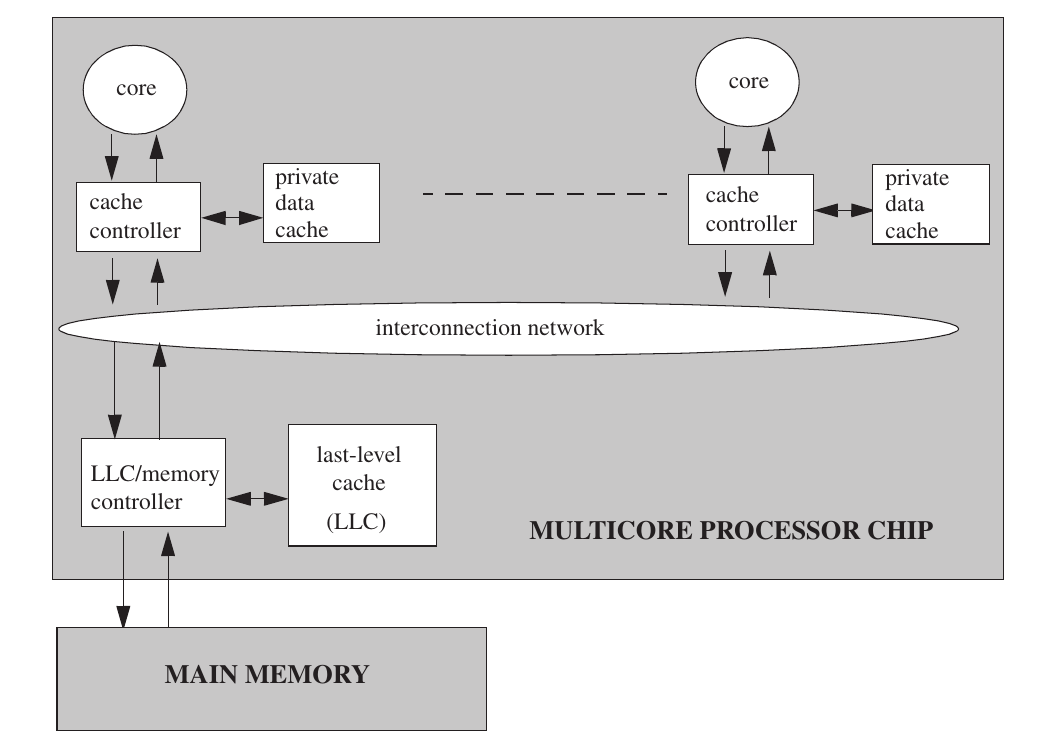
\includegraphics[width=1.\textwidth]{baseline-system}
		\end{column}
		\begin{column}{.6\textwidth}
		基本知识回顾
			\begin{itemize}
				\item 在现代的 CPU(大多数)上,所有的内存访问都需要通过层层的缓存来进行。
				\item 例外:比如,对映射成内存地址的 I/O 口,这些访问至少会绕开这个流程的一部分。
				\item CPU 的读 / 写(以及取指令)单元正常情况下甚至都不能直接访问内存——这是物理结构决定的。
				\item 缓存是分“段”(line)的,一个段对应一块存储空间,大小是 32、64、128字节。
			\end{itemize}
			
		\end{column}
	\end{columns}
	
\end{frame}

%----------------------------------------------
\begin{frame}[plain]	
	\frametitle{Introduction}
	
	
	\begin{columns}
		
		\begin{column}{.4\textwidth}
			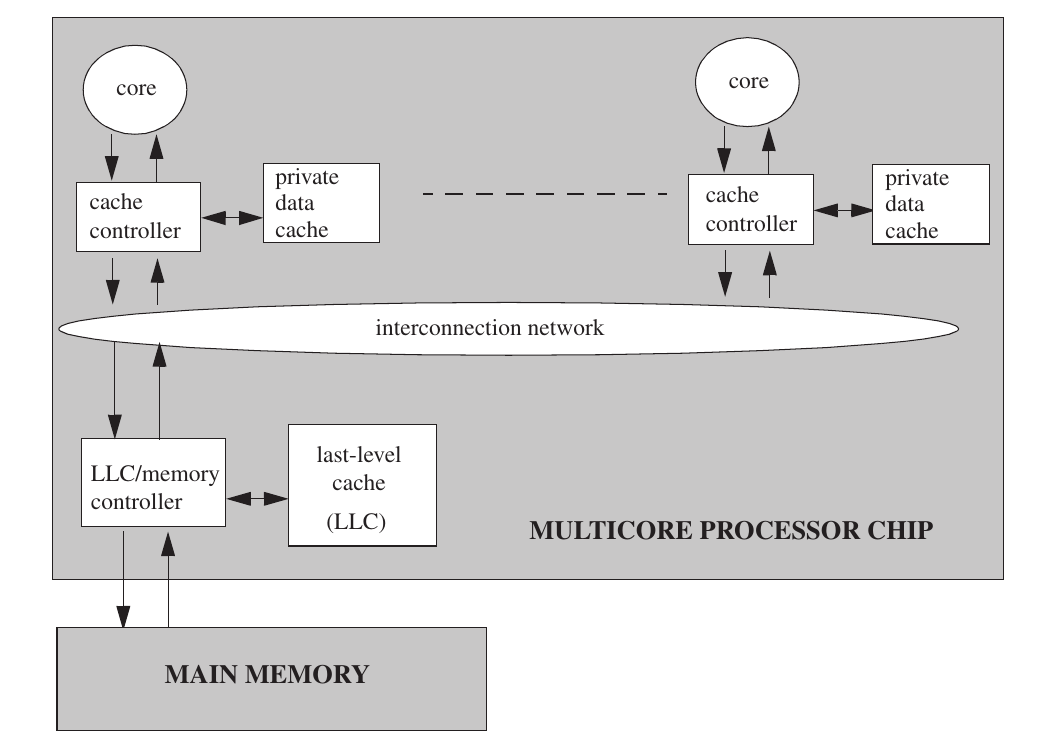
\includegraphics[width=1.\textwidth]{baseline-system}
		\end{column}
		\begin{column}{.6\textwidth}
%			\Large \centering
			回顾 --内存模型(Memory Consistency Model)
			
			Shared-Memory Multi-Core/SMP/NUMA
			
			\begin{itemize}
				\item All cores see a single physical address space
				\item Inter-core communication through loads and stores
				\item Data can be cached in multiple private and shared caches
			\end{itemize}		
			
		\end{column}
	\end{columns}
	
\end{frame}


%----------------------------------------------
\begin{frame}[plain]	
	\frametitle{Introduction}
	
	
	\begin{columns}
		
		\begin{column}{.4\textwidth}
			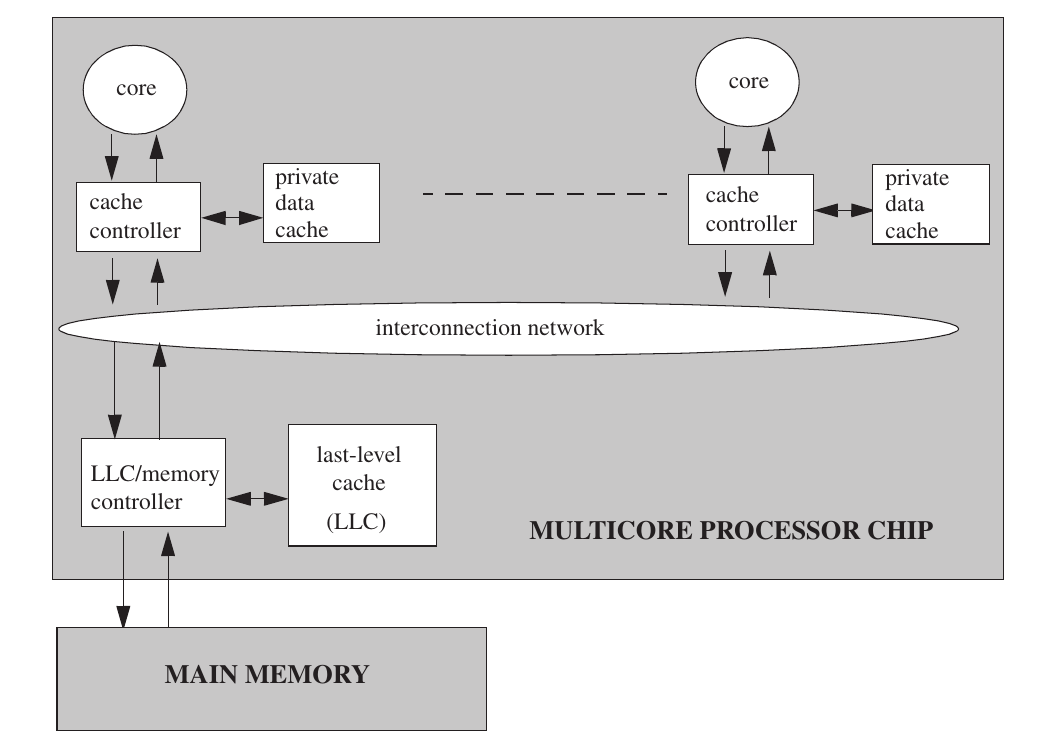
\includegraphics[width=1.\textwidth]{baseline-system}
		\end{column}
		\begin{column}{.6\textwidth}
			%			\Large \centering
			回顾 --内存模型(Memory Consistency Model)
			
			Shared-Memory Multi-Core/SMP/NUMA
			
			Coherence concerns accesses only a single memory location
			\begin{itemize}
				\item Making sure that caches \& stale copies do not cause problems
				\item Two invariants: single-writer multiple-readers, data-value
			\end{itemize}
			\pause
			Consistency concerns ordering for accesses to many locations
			\begin{itemize}
				\item Making sure that ordering does not cause problems
			\end{itemize}			
			
		\end{column}
	\end{columns}
	
\end{frame}

%----------------------------------------------
\begin{frame}[plain]	
	\frametitle{Synchronization}
	
	
	\begin{columns}
		
		\begin{column}{.4\textwidth}
			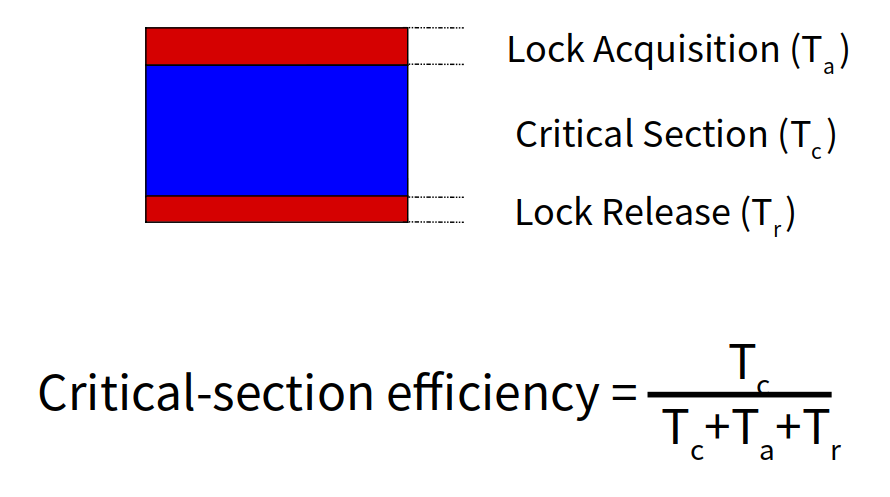
\includegraphics[width=1.\textwidth]{cirtical-section-efficiency}
		\end{column}
		\begin{column}{.6\textwidth}
			%			\Large \centering
			Synchronization requrires mutual exclusion (critical sections)
			
			\begin{itemize}
				\item Acquire (lock)
				\begin{itemize}
					\item Try to obtain the lock or proceed past barrier, may need to wait (spin/busy wait or block)
					\item Must be atomic to both read and write
				\end{itemize}
				\item Release  (unlock)
				\begin{itemize}
					\item Allow other processes to proceed past synchronization event
					
				\end{itemize}				
			\end{itemize}		
			
		\end{column}
	\end{columns}
	
\end{frame}


%----------------------------------------------
\begin{frame}[plain]	
	\frametitle{Atomic Instructions}
	
	
	\begin{columns}
		
		\begin{column}{.4\textwidth}
			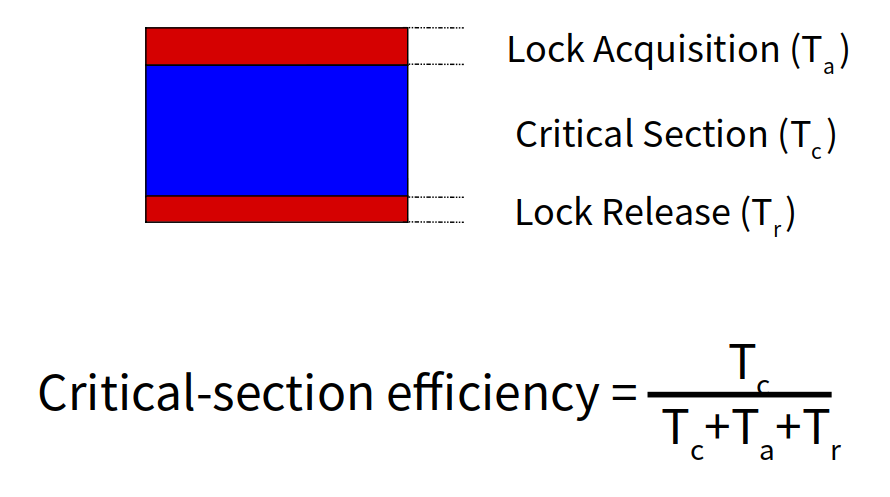
\includegraphics[width=1.\textwidth]{cirtical-section-efficiency}
		\end{column}
		\begin{column}{.6\textwidth}
			%			\Large \centering
			Read-modify-write: specifies an atomic operation on a memory location
			
			\begin{itemize}
				\item Value in memory is read into a register
				\item Another value is written into location
				\begin{itemize}
					\item May or may not depend on the value read
				\end{itemize}
				\item Load and store must happen atomically in hardware
					
			\end{itemize}		
			(Memory Consistency Model
			Many instances
			\begin{itemize}
				\item  Test \& Set
				\item Compare  \&  Swap
				\item Fetch  \& Add/Sub/...				
				
			\end{itemize}		
		\end{column}
	\end{columns}
	
\end{frame}


%----------------------------------------------(Memory Consistency Model
\begin{frame}[fragile]
	\frametitle{Test \& Set}
	
\begin{lstlisting}
boolean test-and-set(*lock)
{
    boolean old=*lock;
    *lock=true;
    return old;
}
\end{lstlisting}
简单互斥算法
\begin{lstlisting}
do
{ while(Test_And_Set_Lock(&lock)); (Memory Consistency Model
  //临界区
  lock = False;
  //剩余区
}while(True)
\end{lstlisting}
\end{frame}
	
    
%----------------------------------------------
\begin{frame}[plain]	
    \frametitle{Improving Performance of Sync}
    
    
    \begin{columns}
        
        \begin{column}{.4\textwidth}
            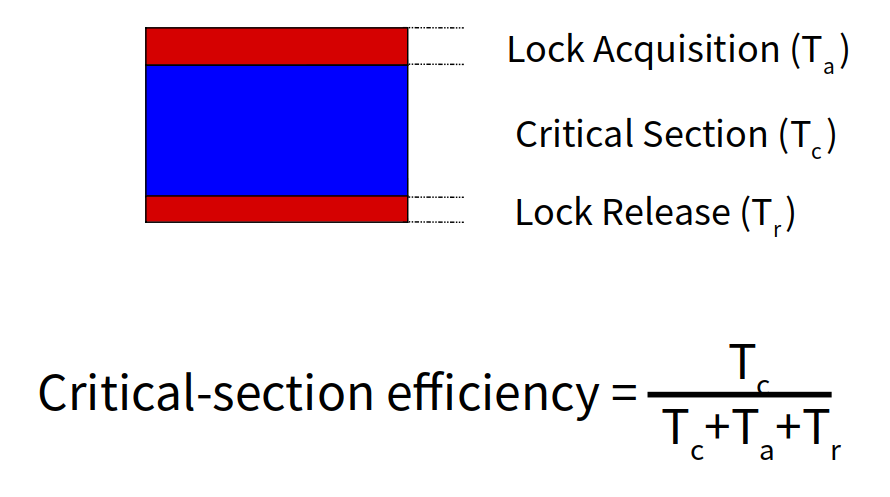
\includegraphics[width=1.\textwidth]{cirtical-section-efficiency}
        \end{column}
        \begin{column}{.6\textwidth}	
            
            Improving Performance of Sync
            \begin{itemize}
                \item Overhead: High contention, read/write miss, ...
                
                \item  Rich interaction of HW-SW tradeoffs
                \item Must evaluate HW primitives and SW algorithms together
                \item Available HW primitives determine which SW algorithms perform well				                
            \end{itemize}		
        \end{column}
    \end{columns}
    
\end{frame}

    
%----------------------------------------------
\begin{frame}[plain]	
    \frametitle{Memory Consistency Model}
    
    \begin{block}{memory consistency model}
        a specification of the allowed    behavior of multithreaded programs executing with shared memory. 
    \end{block} 

    How Core or Cores Might Reorder Memory Accesses
     \begin{itemize}
        \item Store-store reordering: non-FIFO write buffer    
        \item Load-load reordering: C1, C2 dynamically scheduled
        \item Load-store reordering:  Out-of-order cores
        \item Sstore-load reordering:  Out-of-order cores			                
    \end{itemize}
\end{frame}

%----------------------------------------------
\begin{frame}[plain]	
    \frametitle{Memory Consistency Model --  Sequential Consistency}
    
    \begin{block}{Sequential Consistency}
        The result of any         execution is the same as if the operations of all processors (cores) were executed in some sequential         order, and the operations of each individual processor (core) appear in this sequence in the order        specified by its program.
    \end{block} 
    \centering
    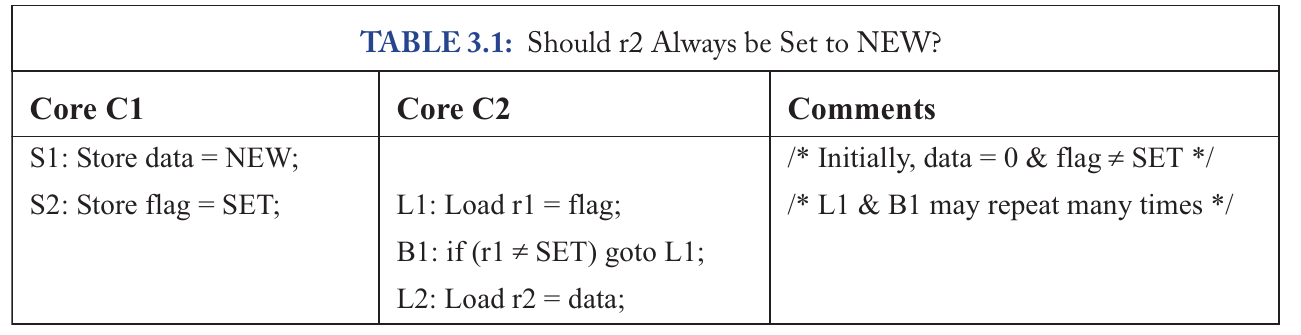
\includegraphics[width=1.\textwidth]{sc-ex1}
    
\end{frame}

%----------------------------------------------
\begin{frame}[plain]	
    \frametitle{Memory Consistency Model --  Sequential Consistency}
    
    \begin{block}{Sequential Consistency}
        The result of any         execution is the same as if the operations of all processors (cores) were executed in some sequential         order, and the operations of each individual processor (core) appear in this sequence in the order        specified by its program.
    \end{block} 
    \centering
    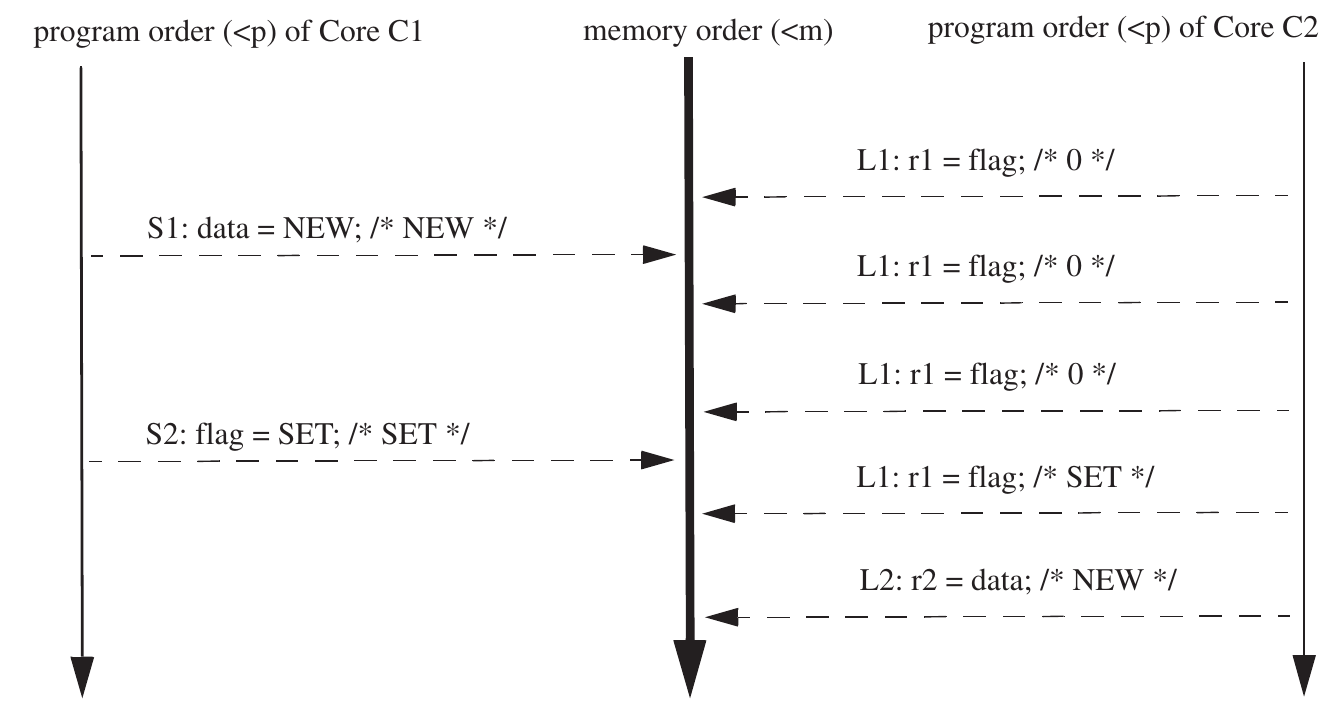
\includegraphics[width=.7\textwidth]{sc-exec1}

\end{frame}

%----------------------------------------------
\begin{frame}[plain]	
    \frametitle{Memory Consistency Model --  Sequential Consistency}
    
    \begin{block}{Sequential Consistency}
        The result of any         execution is the same as if the operations of all processors (cores) were executed in some sequential         order, and the operations of each individual processor (core) appear in this sequence in the order        specified by its program.
    \end{block} 
     
    \begin{itemize}
        \item op1 <p op2 implies that op1 precedes op2 in that core’s program order
        \item op1 <m op2 implies that op1 precedes op2 in memory order.
			                
    \end{itemize}
\end{frame}


%----------------------------------------------
\begin{frame}[plain]	
    \frametitle{Memory Consistency Model --  Sequential Consistency}
    Sequential Consistency execution requires:


    \begin{itemize}
        \item All cores insert their loads and stores into the order <m respecting their program order,
        regardless of whether they are to the same or different addresses (i.e., a=b or a≠b). 
        \begin{itemize}
            \item If L(a) <p L(b) ⇒ L(a) <m L(b) /* Load→Load */
            \item If L(a) <p S(b) ⇒ L(a) <m S(b) /* Load→Store */
            \item If S(a) <p L(b) ⇒ S(a) <m L(b) /* Store→Load */
            \item If S(a) <p S(b) ⇒ S(a) <m S(b) /* Store→Store */

        \end{itemize}
        \pause
        \item Every load gets its value from the last store before it (in global memory order) to the same
        address:
        
        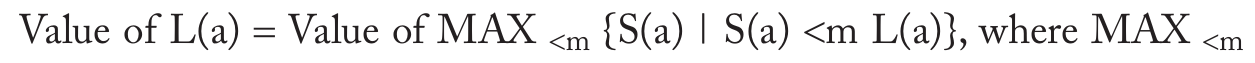
\includegraphics[width=.7\textwidth]{sc-value}
        
        denotes “latest in   memory order.”
        
        \pause
        \item Atomic read–modify–write (RMW) instructions logically appear consecutively in the memory order (no interpose)
        
    \end{itemize}
\end{frame}


%----------------------------------------------
\begin{frame}[plain]	
    \frametitle{Memory Consistency Model --  Sequential Consistency}
The MIPS R10000 [18] provides a venerable, but clean, commercial example for a speculative mi-
croprocessor that implements SC in cooperation with a cache-coherent memory hierarchy.
    
 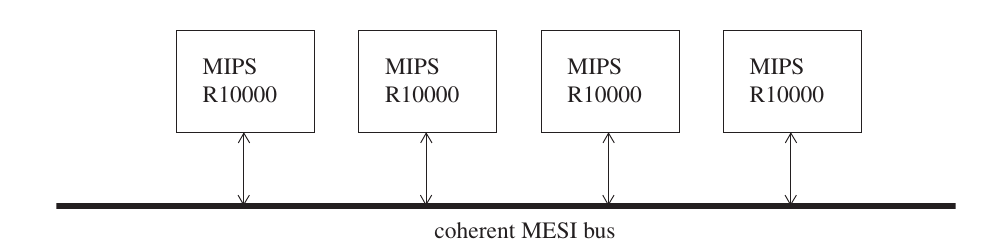
\includegraphics[width=1.\textwidth]{mips-10k}
\end{frame}


%----------------------------------------------
\begin{frame}[plain]	
    \frametitle{Memory Consistency Model --  Total Store Order  Consistency}
   SC本质上要求:
    \begin{itemize}
        \item 缓存一收到总线事件,就可以在当前指令周期中迅速做出响应
        \item 处理器如实地按程序的顺序,把内存操作指令送到缓存,并且等前一条执行完后才能发送下一条
    \end{itemize}
%     \pause
    为了性能,现代处理器无法满足以上条件
    
    \centering
    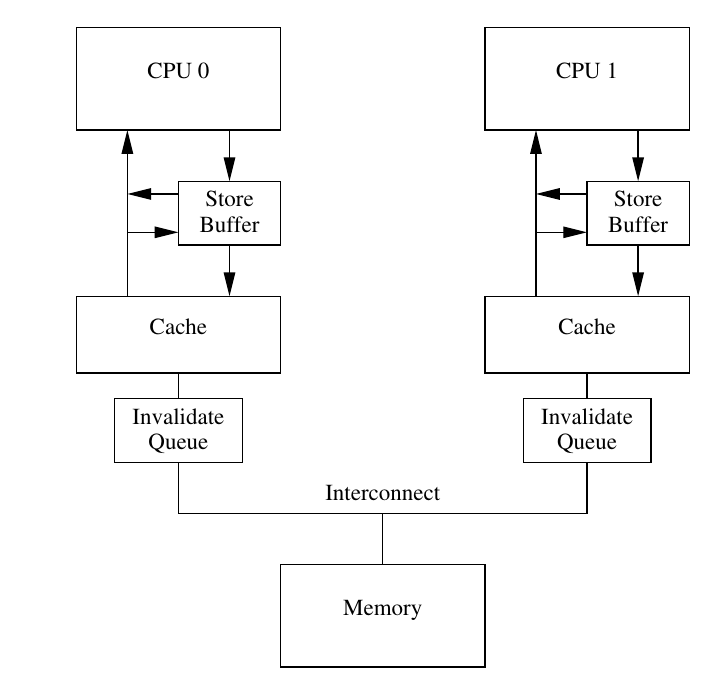
\includegraphics[width=.5\textwidth]{cache-with-wb-iq}
\end{frame}

%----------------------------------------------
\begin{frame}[plain]	
    \frametitle{Memory Consistency Model --  Total Store Order  Consistency}
    为了性能,现代处理器要做到:
    \begin{itemize}
        \item 缓存不会及时响应总线事件。如果总线上发来一条消息,要使某个缓存段失效,但是如果此时缓存正在处理其他事情(比如和 CPU 传输数据),那这个消息可能无法在当前的指令周期中得到处理,而会进入所谓的“失效队列(invalidation queue)”,这个消息等在队列中直到缓存有空为止。

    \end{itemize}
\end{frame}

%----------------------------------------------
\begin{frame}[plain]	
    \frametitle{Memory Consistency Model --  Total Store Order  Consistency}
    为了性能,现代处理器要做到::
    \begin{itemize}
        \item 缓存不会及时响应总线事件。
        \item 处理器一般不会严格按照程序的顺序向缓存发送内存操作指令。当然,有乱序执行(Out-of-Order execution)功能的处理器肯定是这样的。顺序执行(in-order execution)的处理器有时候也无法完全保证内存操作的顺序(比如想要的内存不在缓存中时,CPU 就不能为了载入缓存而停止工作)。
    \end{itemize}
\end{frame}

%----------------------------------------------
\begin{frame}[plain]	
    \frametitle{Memory Consistency Model --  Total Store Order  Consistency}
    为了性能,现代处理器要做到:
    \begin{itemize}
        \item 缓存不会及时响应总线事件。
        \item 处理器一般不会严格按照程序的顺序向缓存发送内存操作指令。
        \item 写操作尤其特殊,因为它分为两阶段操作:在写之前我们先要得到缓存段的独占权。如果我们当前没有独占权,我们先要和其他处理器协商,这也需要一些时间。同理,在这种场景下让处理器闲着无所事事是一种资源浪费。实际上,写操作首先发起获得独占权的请求,然后就进入所谓的由“写缓冲(store buffer)”组成的队列。写操作在队列中等待,直到缓存准备好处理它,此时写缓冲就被“清空(drained)”了,缓冲区被回收用于处理新的写操作。
    \end{itemize}
\end{frame}

%----------------------------------------------
\begin{frame}[plain]	
    \frametitle{Memory Consistency Model --  Total Store Order  Consistency}
    为了性能,现代处理器要做到:
    \begin{itemize}
        \item 缓存不会及时响应总线事件。
        \item 处理器不会严格按照程序的顺序向缓存发送内存操作指令。
        \item 写操作不会严格按照程序的顺序。
    \end{itemize}
这些特性意味着,默认情况下,读操作有可能会读到过时的数据(如果对应失效请求还等在队列中没执行),写操作真正完成的时间有可能比它们在代码中的位置晚,一旦牵涉到乱序执行,一切都变得模棱两可。


\end{frame}

%----------------------------------------------
\begin{frame}[plain]	
    \frametitle{Memory Consistency Model --  Total Store Order  Consistency}
    
%  https://www.cnblogs.com/jiefzz/p/11724765.html
%  如果我们定义store buffer必须严格按照FIFO的次序将数据发送到主存(所谓的FIFO表示先进入store buffer的指令数据必须先于后面的指令数据写到存储器中),这样S3必须要在S1之后执行,CPU能够保证store指令的存储顺序,这种内存模型就叫做完全存储定序(TSO)。
    
    Total Store Order  Consistency (TSO)
   \begin{itemize}
   \item program order v.s. memory order
\begin{itemize}
    \item If L(a) <p L(b) ⇒ L(a) <m L(b) /* Load→Load */
    \item If L(a) <p S(b) ⇒ L(a) <m S(b) /* Load→Store */
    \item If S(a) <p S(b) ⇒ S(a) <m S(b) /* Store→Store */ 
    \item \textbf{NO:} \textit{If S(a) <p L(b) ⇒ S(a) <m L(b) /* Store→Load */}
\end{itemize}
    \item Every load gets its value from the last store before it to the same address:
    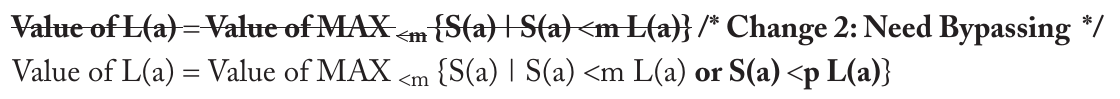
\includegraphics[width=.8\textwidth]{tso-value}
    
    \item \textbf{Fence} orders everything
    \item \textbf{Atomic operations} effectively drain the store buffer
    
\end{itemize}
    
\end{frame}



%----------------------------------------------
\begin{frame}[plain]	
    \frametitle{Memory Consistency Model --  Total Store Order  Consistency}
    QUIZ:
    
    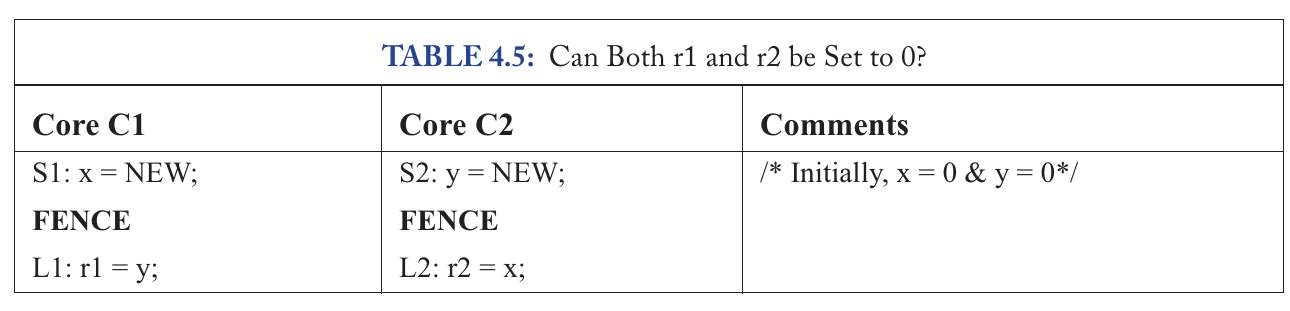
\includegraphics[width=1.\textwidth]{tso-ex1}
    \begin{itemize}
        \item  (x, y) == (0, 0) ? with SC or TSO
        \item delete FENCE ?
        
    \end{itemize}
    \pause
     \begin{itemize}
     \item (x, y) == (0, 0) is not allowed with SC
     \item (x, y) == (0, 0) is possible with TSO :Load bypasses store
     
    \end{itemize}
\end{frame}

%----------------------------------------------
\begin{frame}[plain]	
    \frametitle{Memory Consistency Model --  Total Store Order  Consistency}
    TSO implementation / x86
    
    \begin{itemize}
        \item  x86中,所谓 RMW即 intel 64 架构中的 locked 指令,其包括:隐式 locked 指令如 xchg,也包括别的(助记符中)以 lock 为前缀的 RMW 指令,如 LOCK ADD、LOCK CMPXCHG。这一类指令的特点正如其名,能够使用一个指令完成读取-修改-写入这样复合的行为。
        \pause
        \item locked 指令执行时在总线上断言 LOCK\# signal,这个由处理器提供的信号将为系统总线上锁,此时其它控制该总线的处理器或总线代理将被阻塞。
        \item 作为优化,P6 处理器及之后的处理器型号在执行 locked 指令期间,当访问缓存在处理器内部的内存区域时,将不产生 LOCK\# signal,而采用cache locking,也即更新缓存并依赖缓存一致性算法确保同时仅有一个处理器能修改该内存区域中的数据。
    \end{itemize}
\end{frame}

%----------------------------------------------
\begin{frame}[plain]	
    \frametitle{Memory Consistency Model --  other Consistency}
       Even more relaxed (less ordering)
    \begin{itemize}
        \item  Weak Consistency
        
        \begin{itemize}
            \item Enable higher performance: OoO write buffer, speculation, ...
            \item Need more use of FENCE to enforce ordering
        \end{itemize}   
            
            \item Release Consistency
            \begin{itemize}
            \item ACQUIRE and RELEASE: order memory operations in only one direction
            
            \item ACQUIRE < load, store
            \item Load, store < RELEASE
            \item All ACQUIRE/RELEASE pairs are ordered
       
            \end{itemize}
    \end{itemize}
    
\end{frame}




%-------------------------------------------------
\end{document}